\section{Aufbau und Durchführung}
\label{sec:Durchführung}
Zunächst wurde die Funktionsweise des Signal Processors bzw. Lock-In Amplifier des Lock-In-Verstärkers betrachtet.
Dabei wurden die Spannungsamplituden der Ausgänge Reference und Oscillator
auf Variation bzw. Konstanz mittels eines angeschlossenen digitalen Oszillators hin
überprüft. Der konstante Amplitudenwert wurde notiert.
Anschließend sollte die Schaltung, welche in Abbildung \ref{fig:aufbau1} zu sehen ist, schrittweise aufgebaut werden, wobei der Noise Generator für diesen
Teil ersteinmal überbrückt werden sollte. Zuerst wurde nur ein Sinusförmiges Eingangssignal $U_\text{sig}$ mit einer Frequenz von 1 kHz und einer Spannung von 10 mV auf den
Verstärker gegeben und danach mit einer ebenfalls sinusförmigen Referenzspannung $U_\text{ref}$, gleicher Frequenz, gemischt. Das resultierende Signal wurde auf dem digitalen Oszilloskop
ausgegeben. Für fünf verschiedene Phasen der Referenzspannung, welche am Reference Ausgang einstellbar ist, wurde eine Grafik erstellt.
Anschließend sollte die Schaltung, wie in Abbildung \ref{fig:aufbau1}, vollständig nachgebaut werden, wobei der Noise Generator weiterhin überbrückt wurde.
Nun sollte wieder das Ausgangssignal betrachtet werden, welches nun allerdings integriert wurde, das heißt mit Nutzung des angeschlossenen Tiefpasses. In diesem Aufbau wurden verschiedene Ausgangsspannungen 
in Abhängigkeit von der Phasenverschiebung der Referenzspannung aufgenommen, welche wieder am Reference Ausgang verändert wurde.
In einem nächsten Schritt wurde der Noise Generator wie in Abbildung \ref{fig:aufbau1} angeschlossen. Zu Beachten war, dass sich die vom Noise Generator erzeugten Rauschsignale in der
selben Größenordnung befanden wie die Signalspannung $U_\text{sig}$. Wie schon zuvor wurde nun wieder die Ausgangspannung $U_\text{out}$ in Abhängigkeit der Phasenverschiebung aufgenommen.
\begin{figure}
  \centering
  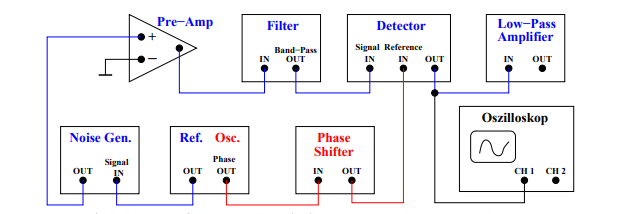
\includegraphics{content/abbildung2.png}
  \caption{Schaltskizze zur Messung der Ausgangspannung in Abhängigkeit zur Phasenverschiebung \cite[4]{V303}}
  \label{fig:aufbau1}
\end{figure}
In einem letzten Schritt sollte der Lock-In-Verstärker auf die Rauschunterdrückung hin untersucht werden.
Hierzu wurde, wie in Abbildung \ref{fig:aufbau2} dargestellt, die Schaltung modifiziert, so dass nun statt des Noise Generators eine LED und eine Photodiode geschaltet sind, welche einen Abstand $r$ von einander haben.
Zu Beachten war, dass die LED mit einer Rechteckspannung versorgt wurde, welche im Frequenzbereich von 50 Hz bis 500 Hz
liegt, weshalb hier mit einer 300 Hz Rechteckspannung gearbeitet wurde. Es wurde die Lichtintensität der LED in Abhängigkeit des veränderlichen Abstandes $r$ gemessen und notiert. Außerdem sollte der maximale Abstand 
$r_\text{max}$ bestimmt werden, an dem das Licht der LED noch mit der Photodiode nachgewiesen werden konnte.
\begin{figure}
  \centering
  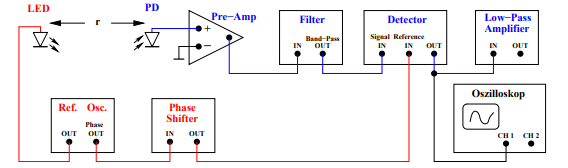
\includegraphics{content/abbildung3.png}
  \caption{Schaltskizze zur Überprüfung der Rauschunterdrückung des Lock-In-Verstärkers mittels einer Photodiode \cite[5]{V303}}
  \label{fig:aufbau2}
\end{figure}